% !TeX root = ../main.tex

\section{Introduzione}
Nei precedenti capitoli sono stati introdotti i concetti alla base della cultura DevOps, del ciclo di vita del processo di sviluppo di applicazioni mobile e delle applicazioni multipiattaforma, arrivando a definire un caso di studio industriale. In questo capitolo viene descritto come è stato effettivamente realizzato il sistema per l'automazione del processo di sviluppo nel rispetto dei requisiti e delle specifiche indicate nel capitolo precedente.

In questa fase di realizzazione del sistema di automazione e di implementazione della pipeline viene considerato il progetto base\footnote{\href{https://github.com/paganellif/DevOps-per-applicazioni-mobile-un-caso-di-studio-industriale/tree/3-applicazioni-multipiattaforma/kmm-example}{https://github.com/paganellif/DevOps-per-applicazioni-mobile-un-caso-di-studio-industriale/tree/3-applicazioni-multipiattaforma/kmm-example}} fornito dal plugin KMM\footnote{\href{https://plugins.jetbrains.com/plugin/14936-kotlin-multiplatform-mobile}{https://plugins.jetbrains.com/plugin/14936-kotlin-multiplatform-mobile}} per Android Studio al fine di mantenere il focus sul processo in modo più agnostico possibile rispetto ad una specifica applicazione utilizzatrice come può essere MaggioliEbook, argomento trattato nel capitolo successivo.

\section{Self-Hosted MacOS GitLab Runner}
% runner macos: in azienda non esistono runner macos.. riprendere il problema del fatto che apple obbliga a usare macOS, indicare le possibili soluzioni (runner managed/self-hosted, ecc) e come ho configurato il runner self-hosted
% approfondire tipologie di runner executor in gitlab e perche ho usato l'executor shell
Come anticipato nel capitolo \ref{ch:app-multiplatform} tutta la toolchain per lo sviluppo iOS è disponibile solamente per il sistema operativo macOS, il che implica la necessità di un ambiente macOS anche per l'esecuzione della pipeline, almeno per tutti i task riguardanti l'applicazione iOS. Esistono diversi modi per realizzare un sistema di automazione compatibile con i vincoli imposti da Apple e possono essere suddivisi nelle seguenti categorie:

\begin{itemize}
    \item \textbf{Soluzione completa as-a-Service} - Il grande interesse per l'automazione e lo sviluppo di applicazioni iOS da parte delle aziende ha portato alla nascita di servizi cloud completamente dedicati a questo scopo come ad esempio \textit{Bitrise}\footnote{\href{https://www.bitrise.io/home}{https://www.bitrise.io/home}} e \textit{XCode Cloud}\footnote{\href{https://developer.apple.com/xcode-cloud/}{https://developer.apple.com/xcode-cloud/}}.
    \item \textbf{Runner macOS managed} - Come anticipato nel capitolo \ref{ch:devops} un runner, ovvero il componente che esegue effettivamente i task della nostra pipeline, può essere \textit{managed} o \textit{self-hosted}. Nel caso di un runner managed con sistema operativo macOS si evita lo sforzo di configurare e mantenere un componente importante del sistema di automazione ma si hanno costi elevati: solitamente al consumo di risorse di questa tipologia di runner è applicato un fattore moltiplicativo poco sostenibile in termini di costi. Alcuni esempi di piattaforme con questo modello di business per i runner managed sono GitHub Action\footnote{\href{https://docs.github.com/en/billing/managing-billing-for-github-actions/about-billing-for-github-actions\#minute-multipliers}{https://docs.github.com/en/billing/managing-billing-for-github-actions/about-billing-for-github-actions\#minute-multipliers}} e GitLab CI\footnote{\href{https://docs.gitlab.com/ee/ci/pipelines/cicd\_minutes.html\#additional-costs-on-gitlab-saas}{https://docs.gitlab.com/ee/ci/pipelines/cicd\_minutes.html\#additional-costs-on-gitlab-saas}}.
    \item \textbf{Runner macOS self-hosted} - L'altra tipologia di runner consiste nella installazione del componente su una macchina con sistema operativo macOS che deve essere configurata e mantenuta dall'utilizzatore. In questo caso è possibile utilizzare macchine virtuali as-a-Service, come quelle fornite da AWS\footnote{\href{https://aws.amazon.com/ec2/instance-types/mac/}{https://aws.amazon.com/ec2/instance-types/mac/}} (Amazon Web Services), oppure hardware fisico Apple per installare ed eseguire il runner.
\end{itemize}

Data la disponibilità di tutta la toolchain Android per macOS e il costo nullo in caso di runner self-hosted, è stata scelta quest'ultima tipologia per l'esecuzione dell'intera pipeline.

L'installazione e la configurazione di un runner di questa tipologia può essere più o meno complicata in base alle funzionalità necessarie per il sistema di automazione. Nel caso specifico del caso di studio di questo progetto l'unica funzionalità richiesta da configurare è la cache condivisa al fine di abilitare la concorrenza tra più processi e ottimizzare l'esecuzione della pipeline.

I seguenti comandi bash\footnote{\href{https://github.com/paganellif/DevOps-per-applicazioni-mobile-un-caso-di-studio-industriale/blob/5-automazione-del-processo-di-sviluppo/setup-gitlab-macos-runner.sh}{https://github.com/paganellif/DevOps-per-applicazioni-mobile-un-caso-di-studio-industriale/blob/5-automazione-del-processo-di-sviluppo/setup-gitlab-macos-runner.sh}} mostrano la procedura di installazione di un runner GitLab macOS self-hosted su una macchina fisica Apple:
\begin{listing}[H]
    \inputminted{bash}{code/macos-runner-setup.sh}
    \caption{Comandi bash per l'installazione, la configurazione e l'avvio di un runner macOS self-hosted}
\end{listing}

Il seguente codice\footnote{\href{https://github.com/paganellif/DevOps-per-applicazioni-mobile-un-caso-di-studio-industriale/blob/5-automazione-del-processo-di-sviluppo/config.toml}{https://github.com/paganellif/DevOps-per-applicazioni-mobile-un-caso-di-studio-industriale/blob/5-automazione-del-processo-di-sviluppo/config.toml}} mostra il file di configurazione del runner, generato in seguito alla procedura sopra indicata:

\begin{listing}[H]
    \inputminted{toml}{code/macos-runner-config.toml}
    \caption{File di configurazione (\textit{config.toml}) generato al momento della installazione del runner}
\end{listing}

\section{Modello di branching}
L’utilizzo di un adeguato flusso di lavoro è fondamentale per definire una efficiente automazione CI/CD. Con branching si intende l’utilizzo di uno o più flussi principali dai quali divergono altri flussi per svolgere determinati lavori per poi convergere al loro termine: in base alle modalità di apertura e chiusura di questi flussi si definiscono diversi modelli di branching.

Il modello che si intende utilizzare (fig. \ref{branching}) è basato sul modello di branching GitFlow\footnote{\href{https://www.atlassian.com/it/git/tutorials/comparing-workflows/gitflow-workflow}{https://www.atlassian.com/it/git/tutorials/comparing-workflows/gitflow-workflow}} e prevede tre branch principali:

\begin{itemize}
    \item \textbf{dev} - Flusso principale di sviluppo. Ogni modifica apportata a questo branch corrisponde al rilascio di una nuova versione \textit{alpha} per la validazione interna. E' da questo branch che vengono aperti e chiusi nuovi branch, sia per lo sviluppo di nuove funzionalità (\textit{feature}) che per la risoluzione di bug/patch (\textit{fix}).

    \begin{figure}[H]
        \centering
        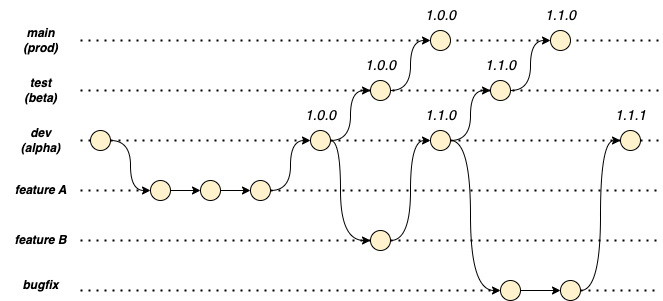
\includegraphics[width=0.65\textwidth]{img/branching-model.png}
        \caption{Esempio di flusso di sviluppo adottando il modello di branching indicato}
        \label{branching}
    \end{figure}
    
    \item \textbf{test} - Branch modificato solamente tramite merge di modifiche provenienti dal branch \textit{dev} con lo scopo di rilasciare una nuova versione \textit{beta} per la validazione esterna.
    \item \textbf{main} - Branch modificato solamente tramite merge di modifiche provenienti dal branch \textit{test} con lo scopo di rilasciare una nuova versione in produzione (\textit{prod}).
\end{itemize}

Grazie ai meccanismi di automazione a supporto della CI/CD fornite dal CI Server si definiscono specifiche regole di attivazione, chiamate \textit{trigger rules}, che permettono di indicare quando uno specifico job deve essere eseguito. Queste regole si basano su eventi che si verificano sul sistema di versionamento come ad esempio commit, tag e merge request. Tramite questa funzionalità è possibile dunque discriminare quali file sono stati modificati e su quale branch per eseguire le operazioni associate come descritto sopra.

\begin{figure}[H]
    \centering
    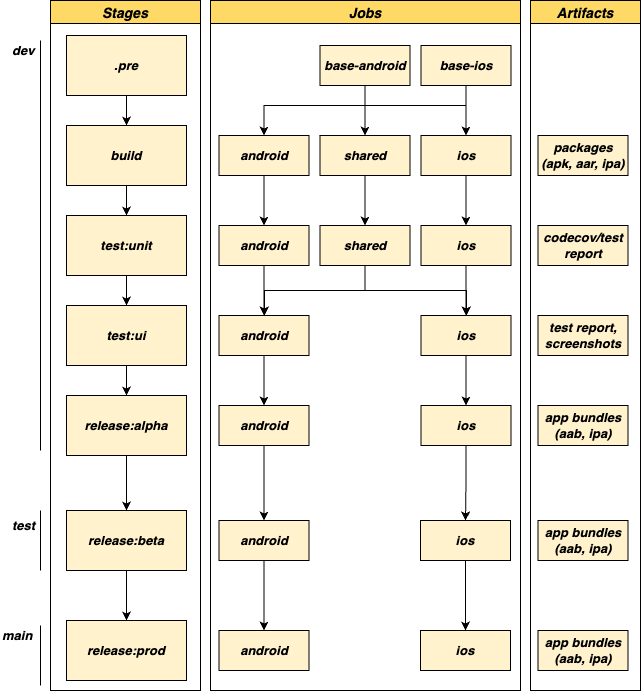
\includegraphics[width=0.85\textwidth]{img/cicd-branch-jobs.png}
    \caption{Stage, job e artefatti associati agli eventi sui branch che compongono l'intera pipeline}
\end{figure}

\section{Templating}
% strumenti utilizzati per favorire il riuso della cicd realizzata

\section{Continuous Integration}
\subsection{Pre}
Molti dei passi che compongono una pipeline utilizzano tipicamente gli stessi tools e le stesse configurazioni per svolgere task diversi. Ad esempio la compilazione del codice e l'esecuzione degli unit test per una applicazione Java utilizzano in entrambi i casi la stessa JDK\footnote{Java Development Kit}, lo stesso tool di build automation e devono essere scaricate le stesse dipendenze di progetto dal package manager di riferimento.

Utilizzando meccanismi di caching e passaggio di artefatti tra i vari job è possibile eseguire tutti quei task di configurazione una sola volta all'inizio della pipeline risparmiando tempo e risorse in tutte le fasi successive.

Nel caso della pipeline progettata per lo sviluppo di applicazioni multipiattaforma con KMM è necessario eseguire i seguenti task di configurazione iniziale:
\begin{itemize}
    \item Configurazione dell'ambiente per lo sviluppo Kotlin tramite l'installazione e il caching degli SDK e del sotto-compilatore \textit{Kotlin/Native}\footnote{\href{https://kotlinlang.org/docs/native-improving-compilation-time.html\#general-recommendations}{https://kotlinlang.org/docs/native-improving-compilation-time.html\#general-recommendations}} per lo sviluppo multipiattaforma.
    \item Configurazione dell'ambiente per lo sviluppo Android tramite l'installazione del SDK Android target e dei vari tools necessari tramite \textit{sdkmanager}\footnote{\href{https://developer.android.com/studio/command-line/sdkmanager}{https://developer.android.com/studio/command-line/sdkmanager}}.
    \item Configurazione dell'ambiente per lo sviluppo iOS tramite impostazione di XCode e CLI Developer Tools.
    \item Installazione e caching di tutte le dipendenze dei vari moduli.
    \item Configurazione delle chiavi per l'autenticazione ai servizi cloud forniti da Google e Apple.
\end{itemize}

Il seguente codice\footnote{\href{https://github.com/paganellif/DevOps-per-applicazioni-mobile-un-caso-di-studio-industriale/blob/5-automazione-del-processo-di-sviluppo/kmm-templates/kmm-base.yml}{https://github.com/paganellif/DevOps-per-applicazioni-mobile-un-caso-di-studio-industriale/blob/5-automazione-del-processo-di-sviluppo/kmm-templates/kmm-base.yml}} mostra il job di pre-configurazione per tutti i job successivi riguardanti la piattaforma Android:

\begin{listing}[H]
    \inputminted{yaml}{code/pre-android-job.yaml}
    \caption{Job di pre-configurazione Android}
\end{listing}

\subsection{Build e Packaging}
Tipicamente la fase di integrazione continua inizia con la verifica della corretta compilazione del codice sorgente. La compilazione rappresenta un vincolo essenziale per tutte le successive fasi e per questo è definita come fase bloccante: in caso di compilazione fallita la pipeline termina senza procedere con le fasi successive definite.

Nel caso dello sviluppo di applicazioni mobile, per lo stage iniziale di build la pratica più diffusa è quella di validare sia la compilazione del codice che la pacchettizzazione della applicazione nei formati richiesti dalle piattaforme target. Dato il funzionamento di una applicazione KMM (Capitolo \ref{ch:app-multiplatform}) è necessario compilare il codice del modulo condiviso \textit{shared} e quello specifico delle piattaforme Android e iOS e impacchettarlo negli artefatti che verranno passati in input alla fase di delivery, rispettivamente aar\footnote{Android Library}, aab e ipa.

Il seguente codice\footnote{\href{https://github.com/paganellif/DevOps-per-applicazioni-mobile-un-caso-di-studio-industriale/blob/5-automazione-del-processo-di-sviluppo/kmm-templates/kmm-build.yml}{https://github.com/paganellif/DevOps-per-applicazioni-mobile-un-caso-di-studio-industriale/blob/5-automazione-del-processo-di-sviluppo/kmm-templates/kmm-build.yml}} mostra il template che definisce il job base di compilazione e pacchettizzazione della applicazione Android tramite l'utilizzo combinato di fastlane e gradle:
\begin{listing}[H]
    \inputminted{yaml}{code/build-job.yaml}
    \caption{Pipeline job dedicato alla compilazione e pacchettizzazione della applicazione Android}
\end{listing}

\subsection{Testing}

\subsection{Dependency Management}

\section{Continuous Delivery}

\subsection{Alpha/Beta Release}

\section{Continuous Inspection}
% progettazione e implementazione analisi
